% Autogenerated translation of quickstart.md by Texpad
% To stop this file being overwritten during the typeset process, please move or remove this header

\documentclass[12pt]{book}
\usepackage{graphicx}
\usepackage{fontspec}
\usepackage[utf8]{inputenc}
\usepackage[a4paper,left=.5in,right=.5in,top=.3in,bottom=0.3in]{geometry}
\setlength\parindent{0pt}
\setlength{\parskip}{\baselineskip}
\setmainfont{Helvetica Neue}
\usepackage{hyperref}
\pagestyle{plain}
\begin{document}

\chapter*{基本使用}

\section*{启动程序}

\subsection*{图形模式}

登陆VN Station后,点击VN Trade Lite快速进入VN Trader(只有CTP接口);或者点击VN Trader Pro先选择如下图的底层接口和上层应用,再进入VN Trader。

\includegraphics{https://vnpy-community.oss-cn-shanghai.aliyuncs.com/forum_experience/yazhang/quick_start/VnTrader_Pro.png}

\subsection*{脚本模式}

在文件夹teststrader中找到run.py文件。按住“Shift” + 鼠标右键进入cmd窗口,输入下面命令进入如图VN Trader
\texttt{
python run.py 
}
\includegraphics{https://vnpy-community.oss-cn-shanghai.aliyuncs.com/forum_experience/yazhang/quick_start/Vntrader.PNG}

~

\section*{连接接口}

以SinNow仿真交易账号登陆CTP接口为例:点击菜单栏的“系统”-$>$“连接CTP”后,弹出如上图所示CTP接口的配置对话框,输入以下内容后即可登录:
- 用户名username:111111 (6位纯数字账号)
- 密码password:1111111  (需要修改一次密码用于盘后测试)
- 经纪商编号brokerid:9999 (SimNow默认经纪商编号)
- 交易服务器地址td\emph{address:180.168.146.187:10030 (盘后测试)
- 行情服务器地址md}address:180.168.146.187:10031 (盘后测试)
- auth\emph{code和product}info主要用于19年中的CTP接入验证,目前留空即可

注意:若使用期货实盘账户,需要问清楚其brokerid、auth\emph{code和product}info; 并且仿真交易需要另外申请开通。

连接成功以后,日志组件会立刻输出陆成功相关信息,同时用户也可以看到账号信息,持仓信息,合约查询等相关信息。

~

\section*{订阅行情}

在交易组件输入交易所和合约代码,并且按“Enter”键即可订阅器行情。如订阅IF股指期货,交易所:CFFEX,名称:IF905;铁矿石期货,交易所:DCE,名称:i1905。

此时行情组件会显示最新行情信息;交易组件会显示合约名称,并且在下方显示深度行情报价:如最新价、买一价、卖一价。(数字货币品种可以显示十档行情)

\includegraphics{https://vnpy-community.oss-cn-shanghai.aliyuncs.com/forum_experience/yazhang/quick_start/subcribe_contract.png}

~

\section*{委托交易}

交易组件适用于手动交易。除了在行情订阅中输入的交易所和合约代码以外,还需要填写以下5个字段:委托方向、开平仓类型、委托类型、委托价格和委托数量。(若委托类型为市价单,委托价格可不填。)

发出委托同时本地缓存委托相关信息,并且显示到委托组件和活动组件,其委托状态为“提交中”,然后等待委托回报。

交易所收到用户发送的委托,将其插入中央订单簿来进行撮合成交,并推送委托回报给用户:
- 若委托还未成交,委托组件和活动组件只会更新时间和委托状态这两字段,委托状态变成“未成交”;
- 若委托立刻成交,委托相关信息会从活动组件移除,新增至成交组件,委托状态变成“全部成交”。

~

\section*{数据监控}

数据监控由以下组件构成,并且附带2个辅助功能:选定以下任一组件,鼠标右键可以选择“调整列宽”(特别适用于屏幕分辨率较低),或者选择“保存数据”(csv格式)

\includegraphics{https://vnpy-community.oss-cn-shanghai.aliyuncs.com/forum_experience/yazhang/quick_start/2_optiones.png}

\subsection*{行情组件}

用于对订阅的行情进行实时监控,如下图,监控内容可以分成3类:

\begin{itemize}
\item 合约信息:合约代码、交易所、合约名称
\item 行情信息:最新价、成交量、开盘价、最高价、最低价、收盘价、买一价、买一量、卖一价、卖一量
\item 其他信息:数据推送时间、接口
\end{itemize}

\includegraphics{https://vnpy-community.oss-cn-shanghai.aliyuncs.com/forum_experience/yazhang/quick_start/subcribe_contract_module.png}

\subsection*{活动组件}

活动组件用于存放还未成交的委托,如限价单或者没有立刻成交的市价单,委托状态永远是“提交中”。在该组件中鼠标双击任一委托可以完成撤单操作。

\includegraphics{https://vnpy-community.oss-cn-shanghai.aliyuncs.com/forum_experience/yazhang/quick_start/active_order.png}

\subsection*{成交组件}

成交组件用于存放已成交的委托,需要注意3个字段信息:价格、数量、时间。他们都是交易所推送过来的成交信息,而不是委托信息。

注意:有些接口会独立推送成交信息,如CTP接口;有些接口则需要从委托信息里面提取成交相关字段,如Tiger接口。

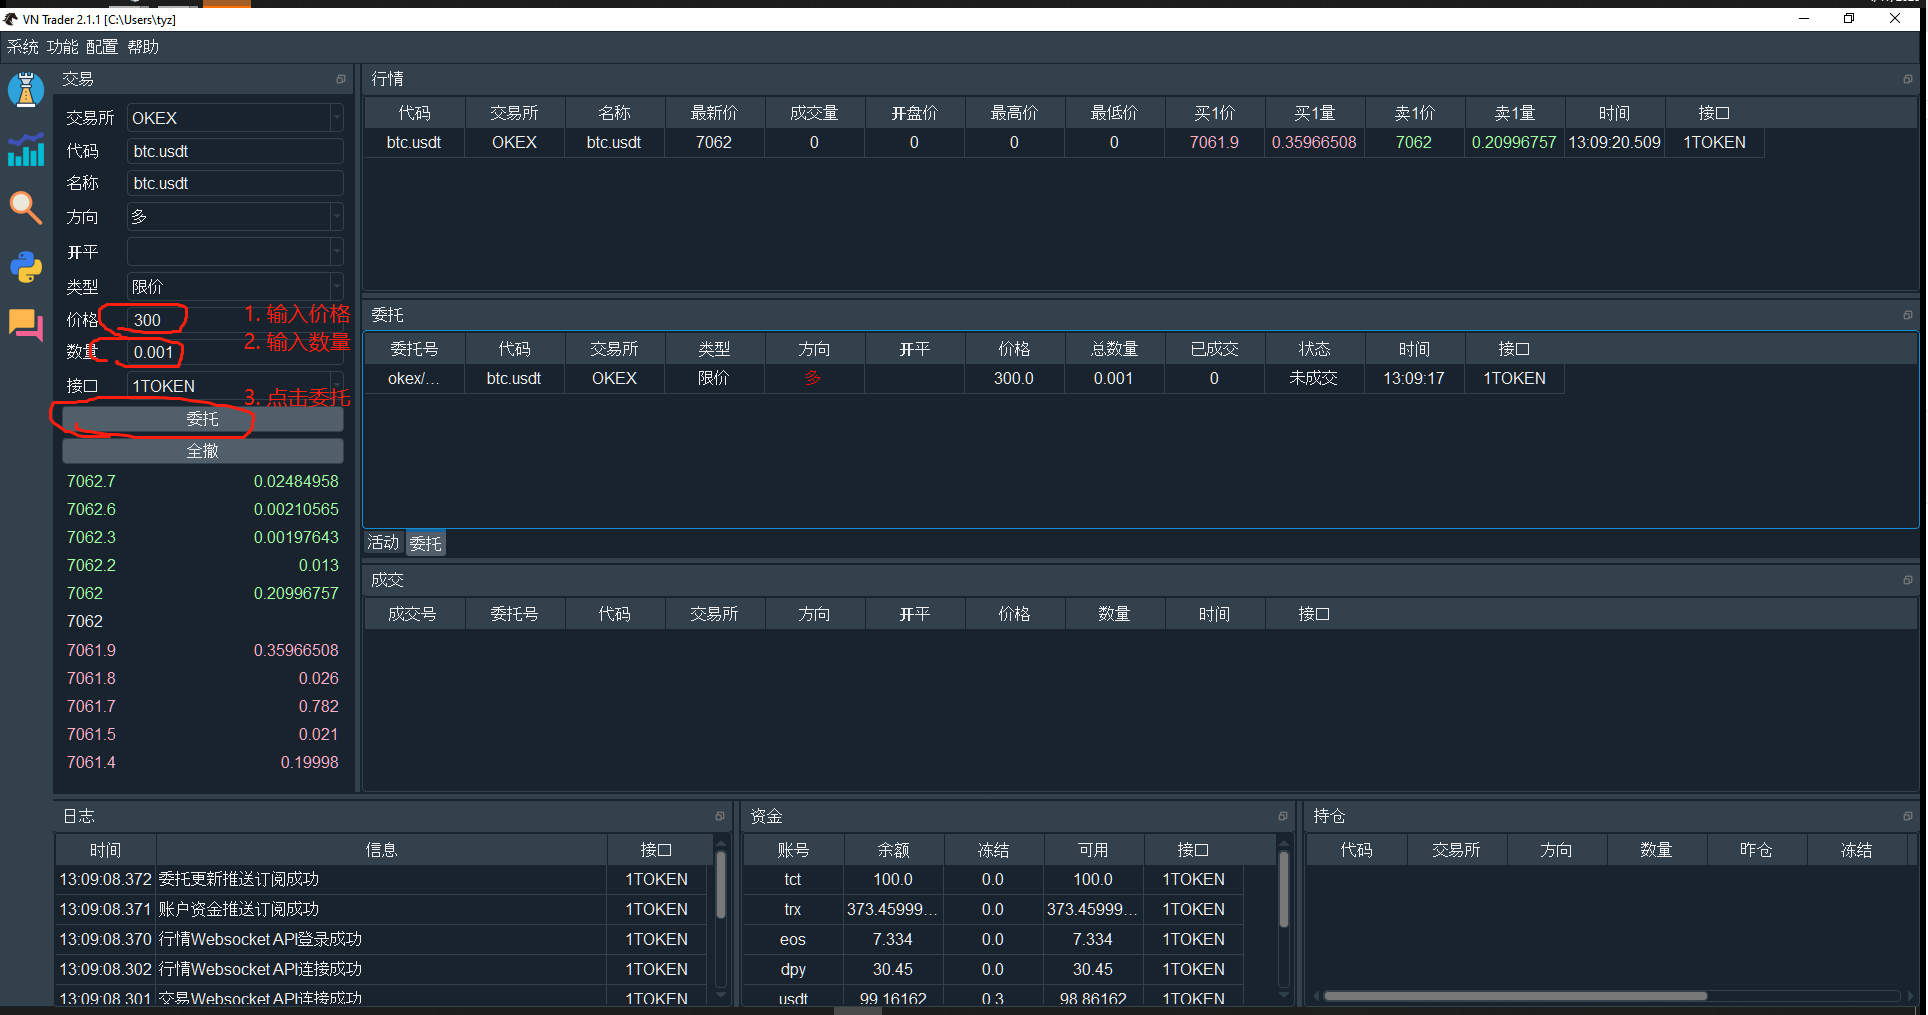
\includegraphics{https://vnpy-community.oss-cn-shanghai.aliyuncs.com/forum_experience/yazhang/quick_start/trade.png}

\subsection*{委托组件}

委托组件用于存放用户发出的所有委托信息,其委托状态可以是提交中、已撤销、部分成交、全部成交、拒单等等。

\includegraphics{https://vnpy-community.oss-cn-shanghai.aliyuncs.com/forum_experience/yazhang/quick_start/order.png}

\subsection*{持仓组件}

持仓组件用于记录其历史持仓。其中需要了解以下字段含义
- 方向:期货品种具有多空方向;而股票品种方向为“净”持仓。
- 昨仓:其出现衍生于上期所特有的平今、平昨模式的需要
- 数量:总持仓,即今仓 + 昨仓
- 均价:历史成交的平均价格(某些巨型委托,会发生多次部分成交,需要计算平均价格)
- 盈亏:持仓盈亏:多仓情况下,盈利 = 当前价格 - 均价;空仓则反之。

若平仓离场,持仓数量清零,浮动盈亏变成实际盈亏从而影响账号余额变化。故以下字段:数量、昨仓、冻结、均价、盈亏均为“0”,如下图。

\includegraphics{https://vnpy-community.oss-cn-shanghai.aliyuncs.com/forum_experience/yazhang/quick_start/query_position.png}

\subsection*{资金组件}

资金组件显示了账号的基础信息,如下图需要注意3个字段信息:
- 可用资金:可以用于委托的现金
- 冻结:委托操作冻结的金额(与保证金不是一个概念)
- 余额:总资金,即可用资金 + 保证金 + 浮动盈亏 

注意:若全部平仓,浮动盈亏变成实际盈亏,保证金和浮动盈亏清零,总资金等于可用资金

\includegraphics{https://vnpy-community.oss-cn-shanghai.aliyuncs.com/forum_experience/yazhang/quick_start/query_account.png}

\subsection*{日志组件}

日志组件用于显示接口登陆信息以及委托报错信息,如下图。

\includegraphics{https://vnpy-community.oss-cn-shanghai.aliyuncs.com/forum_experience/yazhang/quick_start/write_log.png}

~

\section*{应用模块}

vn.py官方提供了开箱即用的量化交易应用模块,在菜单栏中点击“功能”,即显示应用模块,如下图:

\includegraphics{https://vnpy-community.oss-cn-shanghai.aliyuncs.com/forum_experience/yazhang/quick_start/application.png}

\end{document}
